\section{Continuous Integration e Continuous Deployment (CI/CD)}
\label{sect:CICD_it3}
Attraverso le GitHub Actions abbiamo implementato un meccanismo di Continuous Integration e Deployment che ci permette di lavorare sul nostro codice sorgente e non dover provvedere manualmente alla compilazione e pubblicazione dell'immagine Docker con la quale abbiamo pubblicato il nostro backend. La parte di CI avviene direttamente su GitHub, appunto grazie alle Actions, mentre la parte di CD avviene sulla macchina virtuale di Digital Ocean che abbiamo usato per pubblicare l'architettura.
\subsection{Continuous Integration (CI)}
\begin{figure}[h!]
  \centering
  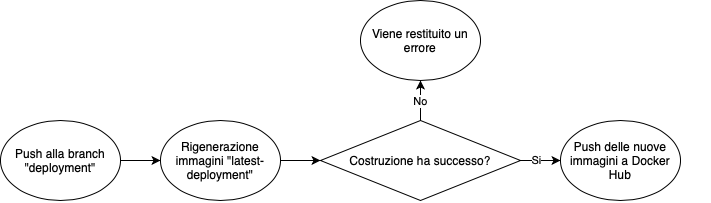
\includegraphics[width=1\textwidth]{Iterazione 3/images/CI.png}
  \caption{Continuous Integration della branch main}
\end{figure}
Il nostro backend è organizzato in 2 immagini:
\begin{enumerate}
  \item \href{https://hub.docker.com/repository/docker/freddy153/ventura-boulevard/}{``ventura-boulevard''}, contenente il manager degli utenti, degli eventi e delle prenotazioni;
  \item \href{https://hub.docker.com/repository/docker/freddy153/radio-nowhere/}{``radio-nowhere''}, contenente l'API Gateway usato per comunicare con la mobile app.
\end{enumerate}
Entrambe le immagini sono organizzate in 2 tag:
\begin{enumerate}
  \item ``latest-development'', l'ultima versione del codice usato per lo sviluppo;
  \item ``latest-deployment'', l'ultima versione del codice usato in produzione e pubblicato su Digital Ocean.
\end{enumerate}
Infine la nostra repository è organizzata attorno a 2 branch principali (oltre a quelle sviluppate al bisogno da ogni membro, ma che non vengono gestite dal sistema CI/CD):
\begin{enumerate}
  \item ``main'', rappresentante la nostra branch di sviluppo, dove poniamo il codice a cui stiamo ancora lavorando ma che non vogliamo pubblicare sul server di produzione;
  \item  ``production'', la nostra branch di produzione, dove è contenuto il codice da cui sono generate le immagini attualmente pubblicate sul server di produzione.
\end{enumerate}
Ad ogni push alla branch main o production vengono rigenerate e ripubblicate su Docker Hub, rispettivamente, l'immagine taggata come ``latest-development'' e \\ ``latest-production''.
Per pubblicare l'immagine compilata sul relativo registry di Docker Hub è necessario accedere con le credenziali del proprietario. Per permette di usarle senza che vengano mai divulgate al pubblico, GitHub mette a disposizione ``Secrets'', che possiamo vedere come un dizionario dove ogni coppia chiave-valore rappresenta una costante che può essere richiamata all'interno delle Actions attraverso la sua chiave. Una volta creata una entry non è più possibile, neppure per l'autore, vederne il contenuto, ma unicamente modificarla o eliminarla.
\newpage
\subsection{Continuous Deployment (CD)}
\label{sect:CD_it3}
\begin{figure}[h!]
  \centering
  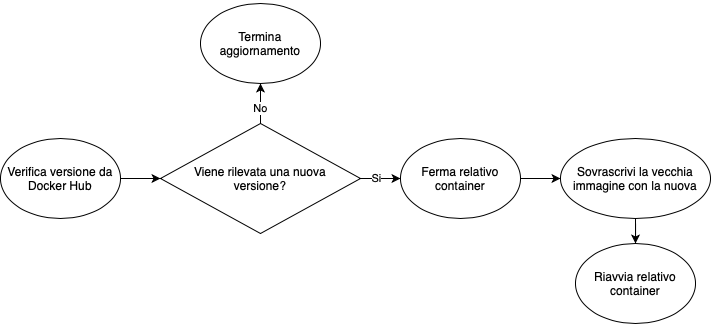
\includegraphics[width=1\textwidth]{Iterazione 3/images/CD.png}
  \caption{Continuous Deployment di un immagine}
\end{figure}
Una volta che l'immagine su Docker Hub è stata rigenerata è necessario che questi cambiamenti vengano rispecchiati sul server di produzione. Per fare ciò abbiamo usato  \href{https://containrrr.dev/watchtower/}{``Watchtower''}, un programma open-source usato per gestire le immagini Docker salvate su una macchina aggiornandole in automatico quando viene pubblicata una nuova versione. Il controllo e l'aggiornamento avvengono a intervalli regolari impostabili dall'utente. Per evitare che il container venisse ricreato troppe volte abbiamo deciso di limitare l'aggiornamento ad una volta al giorno, verso mezzanotte. Rimane poi la possibilità di accedere alla macchina virtuale e riavviare manualmente il container, oppure, scelta meno consigliata, riavviare per intero il server.
